\documentclass[12pt,a4paper]{article}
\usepackage[UTF8]{ctex}
\usepackage{amsmath}
\usepackage{amssymb}
\usepackage{amsthm}
\usepackage{graphicx}
\usepackage{hyperref}
\usepackage{geometry}
\usepackage{listings}
\usepackage{xcolor}
\usepackage{titletoc}
\usepackage{fancyhdr}
\geometry{left=2.5cm,right=2.5cm,top=3cm,bottom=3cm,headheight=15pt}

% 导入通用样式
% 通用样式文件 - 统一所有文档的样式

% 目录样式设置 - 干净简洁,无边框,优化编号
% 使用基本 LaTeX 命令美化目录
\makeatletter
\renewcommand\@dotsep{2}
% 优化编号格式:减少缩进,使编号更紧凑
\renewcommand\l@section{\@dottedtocline{1}{0em}{1.2em}}
\renewcommand\l@subsection{\@dottedtocline{2}{1.2em}{1.8em}}
\renewcommand\l@subsubsection{\@dottedtocline{3}{3em}{2.2em}}
% 设置目录深度为3,显示到subsubsection级别
\setcounter{tocdepth}{3}
\makeatother

% 超链接设置 - 目录链接无颜色框
\hypersetup{
    colorlinks=true,
    linkcolor=black,          % 目录链接为黑色
    filecolor=black,
    urlcolor=blue,
    citecolor=black,
    pdfstartview=FitH,
    pdfborder={0 0 0},        % 无边框
    linkbordercolor={0 0 0},  % 链接边框颜色为黑色(不可见)
    pdfborderstyle={/S/U},    % 无边框样式
}

% 页眉页脚设置(在文档中重新定义)
\usepackage{fancyhdr}
% 注意:每个文档需要在导入 common_style.tex 后设置自己的页眉页脚

% 章节格式 - 简洁美观(使用基本命令)
\makeatletter
\renewcommand\section{\@startsection {section}{1}{\z@}%
                                   {-3.5ex \@plus -1ex \@minus -.2ex}%
                                   {2.3ex \@plus.2ex}%
                                   {\normalfont\Large\bfseries}}
\renewcommand\subsection{\@startsection{subsection}{2}{\z@}%
                                     {-3.25ex\@plus -1ex \@minus -.2ex}%
                                     {1.5ex \@plus .2ex}%
                                     {\normalfont\large\bfseries}}
\renewcommand\subsubsection{\@startsection{subsubsection}{3}{\z@}%
                                     {-3.25ex\@plus -1ex \@minus -.2ex}%
                                     {1.5ex \@plus .2ex}%
                                     {\normalfont\normalsize\bfseries}}
\makeatother

% 代码样式设置 - 简洁干净,无背景色
\definecolor{codegray}{rgb}{0.5,0.5,0.5}
\definecolor{keywordblue}{rgb}{0,0,0.8}
\definecolor{stringred}{rgb}{0.3,0.3,0.3}
\definecolor{commentgreen}{rgb}{0,0.5,0}

\lstdefinestyle{pythonstyle}{
    language=Python,
    % 无背景色 - 使用白色背景,与文档背景一致
    commentstyle=\color{commentgreen},      % 注释不用斜体
    keywordstyle=\color{keywordblue}\bfseries,
    stringstyle=\color{stringred},
    basicstyle=\ttfamily\small,
    breakatwhitespace=false,
    breaklines=true,
    captionpos=b,
    keepspaces=true,
    numbers=none,                           % 不显示行号
    showspaces=false,
    showstringspaces=false,
    showtabs=false,
    tabsize=4,
    frame=single,                          % 保留边框,但更简洁
    rulecolor=\color{black},
    framerule=0.5pt,                       % 细边框
    framexleftmargin=8pt,                  % 左边距(代码与左边框的距离)
    framexrightmargin=8pt,                 % 右边距(代码与右边框的距离)
    framextopmargin=6pt,                   % 上边距(代码与上边框的距离)
    framexbottommargin=6pt,                % 下边距(代码与下边框的距离)
    morekeywords={import,from,as,class,def,return,yield,lambda,if,elif,else,for,while,break,continue,pass,try,except,finally,raise,assert,with,del,global,nonlocal,and,or,not,in,is},
    identifierstyle=\color{black},
}

\lstset{style=pythonstyle}

% 封面宏定义
\newcommand{\makecover}[5]{%
    \newpage
    \thispagestyle{empty}
    \vspace*{1.5cm}
    \begin{center}
        \vspace{2cm}
        {\fontsize{48}{58}\selectfont\bfseries #1}\\[0.8cm]
        \vspace{1.5cm}
        {\Large #2}\\[0.4cm]
        \vspace{1.5cm}
        {\large #3}\\[1.5cm]
        
        % 神经网络图 - 紧凑版本,无标签
        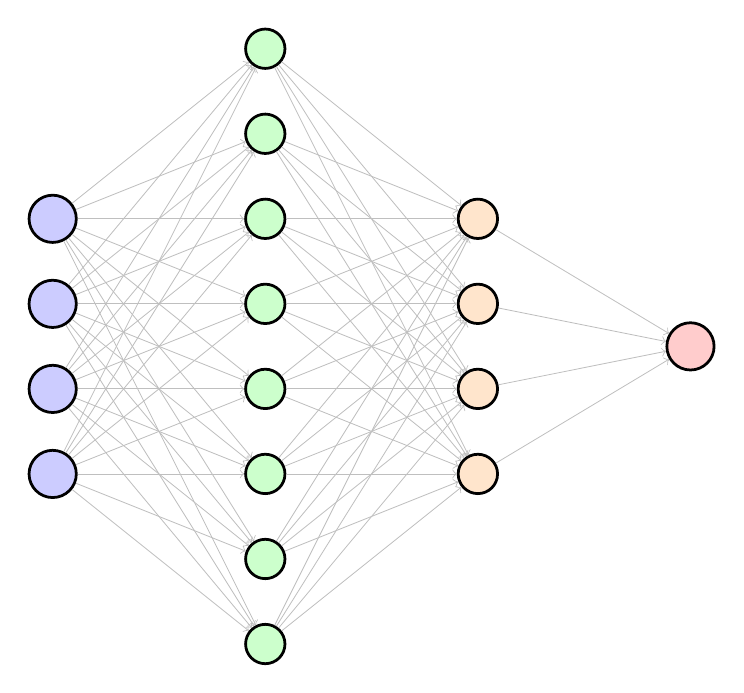
\begin{tikzpicture}[scale=0.9]
        % 定义神经元间距
        \def\spacing{1.2}
        
        % 输入层 - 4个神经元,关于横轴对称
        \node[circle, draw, minimum size=0.6cm, fill=blue!20, line width=1pt] (x1) at (0, -1.8) {};
        \node[circle, draw, minimum size=0.6cm, fill=blue!20, line width=1pt] (x2) at (0, -0.6) {};
        \node[circle, draw, minimum size=0.6cm, fill=blue!20, line width=1pt] (x3) at (0, 0.6) {};
        \node[circle, draw, minimum size=0.6cm, fill=blue!20, line width=1pt] (x4) at (0, 1.8) {};
        
        % 隐藏层1 - 8个神经元,关于横轴对称
        \node[circle, draw, minimum size=0.5cm, fill=green!20, line width=1pt] (h11) at (3, -4.2) {};
        \node[circle, draw, minimum size=0.5cm, fill=green!20, line width=1pt] (h12) at (3, -3.0) {};
        \node[circle, draw, minimum size=0.5cm, fill=green!20, line width=1pt] (h13) at (3, -1.8) {};
        \node[circle, draw, minimum size=0.5cm, fill=green!20, line width=1pt] (h14) at (3, -0.6) {};
        \node[circle, draw, minimum size=0.5cm, fill=green!20, line width=1pt] (h15) at (3, 0.6) {};
        \node[circle, draw, minimum size=0.5cm, fill=green!20, line width=1pt] (h16) at (3, 1.8) {};
        \node[circle, draw, minimum size=0.5cm, fill=green!20, line width=1pt] (h17) at (3, 3.0) {};
        \node[circle, draw, minimum size=0.5cm, fill=green!20, line width=1pt] (h18) at (3, 4.2) {};
        
        % 隐藏层2 - 4个神经元,关于横轴对称
        \node[circle, draw, minimum size=0.5cm, fill=orange!20, line width=1pt] (h21) at (6, -1.8) {};
        \node[circle, draw, minimum size=0.5cm, fill=orange!20, line width=1pt] (h22) at (6, -0.6) {};
        \node[circle, draw, minimum size=0.5cm, fill=orange!20, line width=1pt] (h23) at (6, 0.6) {};
        \node[circle, draw, minimum size=0.5cm, fill=orange!20, line width=1pt] (h24) at (6, 1.8) {};
        
        % 输出层 - 1个神经元,在横轴上
        \node[circle, draw, minimum size=0.6cm, fill=red!20, line width=1pt] (y) at (9, 0) {};
        
        % 输入层到隐藏层1的连接
        \foreach \i in {1,...,4}
            \foreach \j in {1,...,8}
                \draw[->, gray!50, line width=0.3pt] (x\i) -- (h1\j);
        
        % 隐藏层1到隐藏层2的连接
        \foreach \i in {1,...,8}
            \foreach \j in {1,...,4}
                \draw[->, gray!50, line width=0.3pt] (h1\i) -- (h2\j);
        
        % 隐藏层2到输出层的连接
        \foreach \i in {1,...,4}
            \draw[->, gray!50, line width=0.3pt] (h2\i) -- (y);
        \end{tikzpicture}
        
        \vfill
        \vspace{2cm}
        {\normalsize #5}
        \vspace{1.5cm}
    \end{center}
    \newpage
}



% 页眉页脚设置
\pagestyle{fancy}
\fancyhf{}
\fancyhead[L]{\leftmark}
\fancyhead[R]{\thepage}
\fancyfoot[C]{\small AI/ML 综合练习题集}
\renewcommand{\headrulewidth}{0.3pt}
\renewcommand{\footrulewidth}{0.3pt}

\title{AI/ML 综合练习题集}
\author{}
\date{\today}

\newtheorem{definition}{定义}[section]
\newtheorem{example}{例}[section]

\begin{document}

% 封面
\makecover{AI/ML 综合练习题集}{数学基础 · 深度学习 · 大语言模型 · Python 编程}{理论与实践相结合,全面提升 AI/ML 能力}{AI/ML 系列教程}

\maketitle

\tableofcontents
\newpage

\part{数学基础练习题}

\section{计算题}

\subsection{矩阵运算}

\begin{enumerate}
    \item 给定矩阵 $\mathbf{A} = \begin{bmatrix} 1 & 2 \\ 3 & 4 \end{bmatrix}$ 和 $\mathbf{B} = \begin{bmatrix} 5 & 6 \\ 7 & 8 \end{bmatrix}$,计算 $\mathbf{A}\mathbf{B}$、$\mathbf{A}^T$ 和 $\mathbf{A}^{-1}$(如果存在)。
    
    \item 计算向量 $\mathbf{x} = [1, 2, 3]^T$ 的 $L_1$、$L_2$ 和 $L_\infty$ 范数。
    
    \item 给定两个向量 $\mathbf{u} = [1, 0, 1]^T$ 和 $\mathbf{v} = [0, 1, 1]^T$,计算它们的点积和余弦相似度。
\end{enumerate}

\subsection{概率计算}

\begin{enumerate}
    \item 抛一枚公平硬币3次,计算恰好出现2次正面的概率。
    
    \item 假设 $X \sim \mathcal{N}(0, 1)$,计算 $P(-1 < X < 1)$(可以使用标准正态分布表)。
    
    \item 给定先验概率 $P(A) = 0.3$,$P(B|A) = 0.8$,$P(B|\neg A) = 0.2$,使用贝叶斯定理计算 $P(A|B)$。
\end{enumerate}

\subsection{最大似然估计}

\begin{enumerate}
    \item 给定样本 $x_1 = 1, x_2 = 2, x_3 = 3$,假设它们来自泊松分布 $P(X = k) = \frac{\lambda^k e^{-\lambda}}{k!}$,求参数 $\lambda$ 的最大似然估计。
    
    \item 给定样本 $x_1, \ldots, x_n$ 来自指数分布 $p(x) = \lambda e^{-\lambda x}$($x \geq 0$),求参数 $\lambda$ 的最大似然估计。
\end{enumerate}

\subsection{信息论}

\begin{enumerate}
    \item 计算伯努利分布 $P(X=1) = p$,$P(X=0) = 1-p$ 的熵 $H(X)$,并找出使熵最大的 $p$ 值。
    
    \item 给定联合分布:
    \begin{center}
    \begin{tabular}{c|cc}
    $X \backslash Y$ & 0 & 1 \\
    \hline
    0 & 0.3 & 0.2 \\
    1 & 0.1 & 0.4
    \end{tabular}
    \end{center}
    计算 $H(X)$、$H(Y)$、$H(X|Y)$ 和 $I(X; Y)$。
\end{enumerate}

\subsection{优化问题}

\begin{enumerate}
    \item 使用梯度下降法求解 $f(x) = x^2 + 2x + 1$ 的最小值,初始值 $x_0 = 0$,学习率 $\eta = 0.1$,迭代5次。
    
    \item 使用拉格朗日乘数法求解约束优化问题:
    \begin{equation}
    \begin{aligned}
    \min \quad & x^2 + y^2 \\
    \text{s.t.} \quad & x + y = 1
    \end{aligned}
    \end{equation}
\end{enumerate}

\section{概念题}

\subsection{线性代数}

\begin{enumerate}
    \item 解释特征值和特征向量的几何意义。
    
    \item 为什么在机器学习中经常使用矩阵的转置?
    
    \item 解释为什么矩阵乘法不满足交换律,但在神经网络中这通常不是问题。
\end{enumerate}

\subsection{概率论}

\begin{enumerate}
    \item 解释先验概率、似然函数和后验概率的区别和联系。
    
    \item 为什么在机器学习中经常假设误差服从正态分布?
    
    \item 最大似然估计和最大后验估计(MAP)的区别是什么?
\end{enumerate}

\subsection{优化理论}

\begin{enumerate}
    \item 解释为什么梯度下降可能陷入局部最优,而凸优化可以保证全局最优。
    
    \item 学习率的选择对梯度下降有什么影响?
    
    \item 解释拉格朗日乘数的物理意义或几何意义。
\end{enumerate}

\subsection{信息论}

\begin{enumerate}
    \item 解释熵、互信息和 KL 散度的直观含义。
    
    \item 为什么 KL 散度不是真正的距离度量?
    
    \item 在决策树中,为什么使用信息增益而不是直接使用熵?
\end{enumerate}

\subsection{图论}

\begin{enumerate}
    \item 解释邻接矩阵和邻接表的优缺点。
    
    \item 为什么图神经网络需要特殊的消息传递机制,而不能直接使用传统的卷积?
    
    \item 解释图注意力网络中注意力机制的作用。
\end{enumerate}

\section{应用题}

\begin{enumerate}
    \item \textbf{PCA 实现}:
    \begin{itemize}
        \item 给定一个数据矩阵,实现主成分分析(PCA)算法
        \item 使用特征值分解计算主成分
        \item 将数据投影到前两个主成分,可视化结果
    \end{itemize}
    
    \item \textbf{朴素贝叶斯分类器}:
    \begin{itemize}
        \item 实现一个简单的朴素贝叶斯分类器
        \item 在文本分类任务上测试(如垃圾邮件检测)
        \item 分析先验概率对分类结果的影响
    \end{itemize}
    
    \item \textbf{梯度下降可视化}:
    \begin{itemize}
        \item 实现梯度下降算法
        \item 在二维函数上可视化梯度下降的路径
        \item 比较不同学习率对收敛速度的影响
    \end{itemize}
    
    \item \textbf{信息增益计算}:
    \begin{itemize}
        \item 实现信息熵和信息增益的计算
        \item 在简单的数据集上计算各特征的信息增益
        \item 解释为什么信息增益大的特征更适合用于分裂
    \end{itemize}
    
    \item \textbf{图的基本操作}:
    \begin{itemize}
        \item 实现图的邻接矩阵和邻接表表示
        \item 实现图的遍历算法(深度优先搜索、广度优先搜索)
        \item 实现简单的图神经网络消息传递
    \end{itemize}
\end{enumerate}

\section{综合思考题}

\begin{enumerate}
    \item \textbf{数学工具的综合应用}:
    \begin{itemize}
        \item 选择一个机器学习算法(如逻辑回归、支持向量机、神经网络),分析其中用到了哪些数学工具。
        \item 解释这些数学工具在算法中各自的作用。
        \item 讨论如果缺少某个数学工具,算法会如何变化。
    \end{itemize}
    
    \item \textbf{数学与直觉}:
    \begin{itemize}
        \item 选择一个数学概念(如熵、梯度、特征值),用非数学的语言解释其直观含义。
        \item 举一个生活中的例子说明这个概念。
        \item 解释这个概念在机器学习中的重要性。
    \end{itemize}
    
    \item \textbf{数学证明}:
    \begin{itemize}
        \item 证明信息熵的非负性。
        \item 证明 KL 散度的非负性(使用 Jensen 不等式)。
        \item 证明梯度指向函数值增加最快的方向。
    \end{itemize}
\end{enumerate}

\part{深度学习练习题}

\section{概念题}

\begin{enumerate}
    \item \textbf{梯度消失问题}:
    \begin{itemize}
        \item 解释什么是梯度消失问题,为什么会出现?
        \item 列举至少三种缓解梯度消失问题的方法,并说明其原理。
        \item 为什么 ReLU 激活函数能够缓解梯度消失问题?
    \end{itemize}
    
    \item \textbf{卷积神经网络}:
    \begin{itemize}
        \item 解释卷积操作中的局部连接和权重共享如何减少参数量。
        \item 比较最大池化和平均池化的优缺点。
        \item 为什么 CNN 适合处理图像数据?
    \end{itemize}
    
    \item \textbf{注意力机制}:
    \begin{itemize}
        \item 解释自注意力和交叉注意力的区别。
        \item 为什么 Transformer 需要位置编码?
        \item 多头注意力的优势是什么?
    \end{itemize}
    
    \item \textbf{批量归一化}:
    \begin{itemize}
        \item 解释批量归一化为什么能够加速训练。
        \item 批量归一化在训练和测试阶段的区别是什么?
        \item 为什么批量归一化具有正则化效果?
    \end{itemize}
    
    \item \textbf{强化学习}:
    \begin{itemize}
        \item 解释强化学习与监督学习的区别。
        \item 什么是探索-利用权衡(Exploration-Exploitation Trade-off)?
        \item DQN 中的经验回放和目标网络的作用是什么?
    \end{itemize}
    
    \item \textbf{损失函数}:
    \begin{itemize}
        \item 比较均方误差(MSE)和平均绝对误差(MAE)的优缺点,各适用于什么场景?
        \item 为什么交叉熵损失函数与 softmax 激活函数配合使用效果最佳?
        \item 解释 Focal Loss 如何解决类别不平衡问题,其核心思想是什么?
        \item 在什么情况下应该使用 Huber Loss 而不是 MSE 或 MAE?
        \item 三元组损失函数在度量学习中的作用是什么?如何选择正负样本?
    \end{itemize}
\end{enumerate}

\section{编程题}

\begin{enumerate}
    \item \textbf{实现多层感知机}:
    \begin{itemize}
        \item 使用 PyTorch 或 TensorFlow 实现一个三层 MLP(输入层、隐藏层、输出层)
        \item 在 MNIST 数据集上训练模型
        \item 实现前向传播和反向传播(可以调用框架的自动微分功能)
        \item 尝试不同的激活函数(Sigmoid、tanh、ReLU)并比较效果
    \end{itemize}
    
    \item \textbf{实现简单的 CNN}:
    \begin{itemize}
        \item 实现一个包含卷积层、池化层和全连接层的 CNN
        \item 在 CIFAR-10 数据集上训练模型
        \item 可视化卷积层的特征图,观察不同层学习到的特征
    \end{itemize}
    
    \item \textbf{实现 LSTM}:
    \begin{itemize}
        \item 使用 PyTorch 或 TensorFlow 实现 LSTM 单元
        \item 在文本分类任务(如情感分析)上训练模型
        \item 比较 LSTM 和简单 RNN 的性能差异
    \end{itemize}
    
    \item \textbf{实现注意力机制}:
    \begin{itemize}
        \item 实现自注意力机制
        \item 实现多头注意力机制
        \item 在序列到序列任务(如机器翻译)中应用注意力机制
    \end{itemize}
    
    \item \textbf{实现批量归一化}:
    \begin{itemize}
        \item 实现批量归一化层(包括训练和测试模式)
        \item 在深度网络中应用批量归一化,观察训练速度和最终性能的变化
        \item 比较使用和不使用批量归一化的训练曲线
    \end{itemize}
    
    \item \textbf{实现 Dropout}:
    \begin{itemize}
        \item 实现 Dropout 层(包括训练和测试模式)
        \item 在过拟合的模型上应用 Dropout,观察正则化效果
        \item 可视化 Dropout 对模型权重分布的影响
    \end{itemize}
    
    \item \textbf{实现不同的损失函数}:
    \begin{itemize}
        \item 实现 MSE、MAE 和 Huber Loss,比较它们在回归任务上的表现
        \item 实现交叉熵损失函数,在分类任务上验证其效果
        \item 实现 Focal Loss,在类别不平衡的数据集上比较其与标准交叉熵的差异
        \item 实现三元组损失函数,在图像检索任务中应用
        \item 尝试组合多个损失函数(如内容损失 + 风格损失),观察效果
    \end{itemize}
\end{enumerate}

\section{综合项目}

\subsection{项目:图像分类系统}

\begin{itemize}
    \item 使用深度学习框架(PyTorch 或 TensorFlow)构建一个完整的图像分类系统
    \item 实现数据加载、预处理、模型定义、训练和评估的完整流程
    \item 尝试不同的网络架构(MLP、CNN、ResNet)
    \item 应用不同的优化技术(批量归一化、Dropout、学习率调度)
    \item 使用数据增强技术提高模型泛化能力
    \item 可视化训练过程(损失曲线、准确率曲线)
    \item 分析模型的错误案例,提出改进方案
\end{itemize}

\subsection{项目:文本生成系统}

\begin{itemize}
    \item 使用 RNN/LSTM/GRU 或 Transformer 构建文本生成模型
    \item 在文本数据集(如小说、新闻)上训练模型
    \item 实现不同的采样策略(贪婪搜索、随机采样、束搜索)
    \item 评估生成文本的质量(困惑度、BLEU 分数等)
    \item 尝试不同的超参数设置,观察对生成质量的影响
\end{itemize}

\subsection{项目:强化学习智能体}

\begin{itemize}
    \item 使用深度强化学习(DQN 或策略梯度方法)训练游戏智能体
    \item 在 OpenAI Gym 环境(如 CartPole、Atari 游戏)中训练
    \item 实现经验回放和目标网络(对于 DQN)
    \item 可视化训练过程和智能体的行为
    \item 分析不同超参数(学习率、折扣因子等)对性能的影响
\end{itemize}

\section{研究性作业}

\begin{enumerate}
    \item \textbf{文献阅读}:阅读以下经典论文,总结其主要贡献:
    \begin{itemize}
        \item LeCun et al. (1998). "Gradient-based learning applied to document recognition"
        \item Krizhevsky et al. (2012). "ImageNet classification with deep convolutional neural networks"
        \item He et al. (2016). "Deep residual learning for image recognition"
        \item Vaswani et al. (2017). "Attention is all you need"
        \item Devlin et al. (2018). "BERT: Pre-training of deep bidirectional transformers for language understanding"
    \end{itemize}
    
    \item \textbf{技术调研}:选择一个深度学习应用领域(如医疗影像、自动驾驶、金融风控),调研该领域的最新进展,包括:
    \begin{itemize}
        \item 主要技术方法
        \item 面临的挑战
        \item 最新研究成果
        \item 实际应用案例
    \end{itemize}
    
    \item \textbf{实验设计}:设计一个实验来验证某个深度学习技术(如批量归一化、残差连接)的有效性:
    \begin{itemize}
        \item 明确研究问题
        \item 设计对比实验
        \item 确定评估指标
        \item 分析实验结果
    \end{itemize}
\end{enumerate}

\part{大语言模型练习题}

\section{概念题}

\begin{enumerate}
    \item \textbf{Transformer 架构}:
    \begin{itemize}
        \item 解释自注意力和交叉注意力的区别。
        \item 为什么 Transformer 需要位置编码?
        \item 多头注意力的优势是什么?
    \end{itemize}
    
    \item \textbf{预训练与微调}:
    \begin{itemize}
        \item 比较自回归语言建模和掩码语言建模的优缺点。
        \item 解释 Few-shot Learning 和 In-context Learning 的区别。
        \item LoRA 如何实现参数高效微调?
    \end{itemize}
    
    \item \textbf{提示工程}:
    \begin{itemize}
        \item Chain-of-Thought 如何提高模型的推理能力?
        \item Few-shot Prompting 的工作原理是什么?
        \item 如何设计有效的提示?
    \end{itemize}
    
    \item \textbf{RAG}:
    \begin{itemize}
        \item RAG 相比直接生成有什么优势?
        \item 如何构建高效的检索系统?
        \item RAG 如何解决大模型的幻觉问题?
    \end{itemize}
\end{enumerate}

\section{编程题}

\begin{enumerate}
    \item \textbf{实现 Transformer 编码器}:
    \begin{itemize}
        \item 使用 PyTorch 实现完整的 Transformer 编码器
        \item 包含位置编码、多头注意力、前馈网络
        \item 在文本分类任务上测试
    \end{itemize}
    
    \item \textbf{实现注意力机制}:
    \begin{itemize}
        \item 实现缩放点积注意力
        \item 实现多头注意力
        \item 可视化注意力权重
    \end{itemize}
    
    \item \textbf{实现 RAG 系统}:
    \begin{itemize}
        \item 构建文档向量索引
        \item 实现检索功能
        \item 基于检索结果生成答案
    \end{itemize}
    
    \item \textbf{提示工程实践}:
    \begin{itemize}
        \item 设计 Few-shot Prompting 提示
        \item 实现 Chain-of-Thought 提示
        \item 比较不同提示策略的效果
    \end{itemize}
    
    \item \textbf{模型微调}:
    \begin{itemize}
        \item 使用 Hugging Face Transformers 微调预训练模型
        \item 实现 LoRA 微调
        \item 比较全参数微调和 LoRA 的效果
    \end{itemize}
\end{enumerate}

\section{综合项目}

\subsection{项目:构建智能问答系统}

\begin{itemize}
    \item 使用预训练的大语言模型
    \item 实现 RAG 增强生成
    \item 构建知识库和检索系统
    \item 设计用户界面
    \item 评估系统性能
\end{itemize}

\subsection{项目:代码生成助手}

\begin{itemize}
    \item 在代码数据集上微调模型
    \item 实现代码生成功能
    \item 添加代码补全功能
    \item 实现代码审查功能
\end{itemize}

\part{大语言模型先进技术练习题}

\section{概念理解题}

\begin{enumerate}
    \item 解释 LoRA 的数学原理,说明为什么低秩分解能够有效。
    
    \item 比较 QLoRA 和 LoRA 的区别,说明量化的作用。
    
    \item 解释 Flash Attention 如何减少内存占用。
    
    \item 说明 BLEU 分数的简短惩罚的作用。
    
    \item 解释 ROUGE-L 和 ROUGE-N 的区别。
\end{enumerate}

\section{计算题}

\begin{enumerate}
    \item \textbf{困惑度计算}:
    \begin{itemize}
        \item 给定序列长度为 100,平均对数概率为 -2.5,计算困惑度
        \item 手算并编写代码验证
    \end{itemize}
    
    \item \textbf{BLEU 计算}:
    \begin{itemize}
        \item 参考:\texttt{"the cat sat on the mat"}
        \item 候选:\texttt{"a cat sat on mat"}
        \item 计算 1-gram 到 4-gram 的精确度、简短惩罚和 BLEU 分数
        \item 手算并编写代码验证
    \end{itemize}
    
    \item \textbf{ROUGE 计算}:
    \begin{itemize}
        \item 参考:\texttt{"the cat is on the mat"}
        \item 候选:\texttt{"cat mat"}
        \item 计算 ROUGE-1、ROUGE-2 和 ROUGE-L
        \item 手算并编写代码验证
    \end{itemize}
\end{enumerate}

\section{代码实现题}

\begin{enumerate}
    \item 实现一个完整的 LoRA 训练脚本,包括数据加载、模型配置、训练循环和评估。
    
    \item 实现 BLEU 分数计算函数,支持多个参考文本。
    
    \item 实现 ROUGE 分数计算函数,包括 ROUGE-N 和 ROUGE-L。
    
    \item 实现困惑度计算函数,支持批量计算。
\end{enumerate}

\section{案例分析题}

\begin{enumerate}
    \item 给定一个文本生成任务,设计完整的评估方案,包括选择合适的评估指标、实现评估代码、分析结果。
    
    \item 分析 LoRA 在不同任务上的效果,比较不同 rank 设置的影响。
    
    \item 设计一个模型部署方案,包括模型压缩、服务化部署和性能优化。
\end{enumerate}

\part{Python/NumPy/Pandas 练习题}

\section{NumPy 综合例题}

\subsection{例题1:数据预处理}

给定一个包含1000个样本、20个特征的数据集,完成以下任务:
\begin{enumerate}
    \item 计算每个特征的均值和标准差
    \item 进行Z-score标准化(均值为0,标准差为1)
    \item 检测并处理异常值(使用3σ原则)
    \item 将数据重塑为适合输入神经网络的形状
\end{enumerate}

\subsection{例题2:矩阵运算与线性代数}

给定矩阵 $\mathbf{A} = \begin{bmatrix} 1 & 2 & 3 \\ 4 & 5 & 6 \end{bmatrix}$ 和向量 $\mathbf{b} = \begin{bmatrix} 1 \\ 2 \\ 3 \end{bmatrix}$,完成以下任务:
\begin{enumerate}
    \item 计算矩阵乘法 $\mathbf{A}\mathbf{b}$
    \item 计算 $\mathbf{A}$ 的转置 $\mathbf{A}^T$
    \item 计算 $\mathbf{A}^T\mathbf{A}$ 的特征值和特征向量
    \item 对 $\mathbf{A}$ 进行SVD分解
\end{enumerate}

\subsection{例题3:统计分析与数据探索}

给定一个包含学生成绩的数据集,完成以下分析:
\begin{enumerate}
    \item 计算各科目的平均分、标准差、最高分、最低分
    \item 找出总分最高的学生
    \item 计算各科目的及格率(60分以上)
    \item 找出所有科目都及格的学生
\end{enumerate}

\subsection{例题4:广播机制的实际应用}

实现批量归一化(Batch Normalization)操作,这是深度学习中常用的技术。

要求:
\begin{enumerate}
    \item 给定一个批次的数据 $\mathbf{X} \in \mathbb{R}^{B \times D}$($B$ 个样本,$D$ 个特征)
    \item 对每个特征进行归一化:$\hat{x}_i = \frac{x_i - \mu}{\sigma}$
    \item 应用缩放和平移:$y_i = \gamma \hat{x}_i + \beta$
\end{enumerate}

\section{编程实践题}

\begin{enumerate}
    \item \textbf{数组操作}:
    \begin{itemize}
        \item 创建一个 $5 \times 5$ 的随机数组
        \item 提取对角线元素
        \item 计算每行的均值和标准差
        \item 找出最大值和最小值的位置
    \end{itemize}
    
    \item \textbf{广播机制应用}:
    \begin{itemize}
        \item 给定一个 $100 \times 10$ 的特征矩阵
        \item 使用广播机制对每个特征进行标准化
        \item 验证标准化后的均值和标准差
    \end{itemize}
    
    \item \textbf{线性代数运算}:
    \begin{itemize}
        \item 实现矩阵乘法的多种方法
        \item 计算矩阵的逆和行列式
        \item 实现特征值分解和SVD分解
    \end{itemize}
    
    \item \textbf{统计分析}:
    \begin{itemize}
        \item 生成模拟数据
        \item 计算各种统计量(均值、方差、中位数、百分位数)
        \item 检测和处理异常值
    \end{itemize}
\end{enumerate}

\section{综合项目}

\textbf{项目:数据预处理流水线}

\begin{itemize}
    \item 实现一个完整的数据预处理流水线
    \item 包括数据加载、清洗、特征工程、标准化等步骤
    \item 使用 NumPy 进行高效的数值计算
    \item 可视化数据分布和预处理效果
    \item 评估预处理对后续机器学习任务的影响
\end{itemize}

通过完成以上练习题,读者可以全面掌握 AI/ML 领域的核心知识,从数学基础到深度学习,从大语言模型到实际应用,建立完整的知识体系。

\end{document}

